\documentclass[pdftex,a4paper]{extarticle}
\usepackage[utf8]{inputenc}

\title{Functional Reactive Programming and it`s application in Functional Game Programming}
\author{{\large David Kraeutmann, Phillip Kindermann} \\
{\em RWTH Aachen}}

\usepackage{natbib}
\usepackage{graphicx}
\usepackage{url}
\usepackage{amsmath}
\usepackage{amssymb}
\usepackage{amsthm}
\usepackage{enumitem}
\usepackage{minted}
\usepackage{parcolumns}
\usepackage[normalem]{ulem}
\usepackage{multicol}
\usepackage{caption}
\usepackage[a4paper]{geometry}

\usepackage{tikz}
\usetikzlibrary{shapes,snakes}
\usetikzlibrary{scopes,backgrounds}

\tikzset{signal function/.style={draw=black, rectangle, minimum width=6em}}
\tikzset{signal function with state/.style={draw=black, rectangle split, rectangle split parts = 2, rectangle split draw splits = false, minimum width=6em}}

\usepackage{fancyvrb}
\DefineShortVerb{\|}

\begin{document}
\maketitle

\section{Introduction}
Real-time programming is at its core quite imperative --- read input, update state, write output, repeat. 
That requires you to describe \emph{what to do} instead of \emph{what you want}, which leads to a lot of boilerplate when just trying to model a state update.
However, without additional thought even programs written using declarative programming lose their unique benefits due to the imperative style imposed by the update loop, large amounts of state and discrete-time semantics. 
\begin{listing}[ht]
\inputminted[breaklines=true]{haskell}{../vortrag_david/Loop.hs}
\captionof{listing}{Update loop of a Haskell program}
\label{lst:imperative}
\end{listing}

To address these issues, Elliott/Hudak formulated \emph{Functional Reactive Programming} (FRP) in \cite{ElliottHudak97:Fran}. FRP evolved in a myriad of different directions and has  applications in robotics, computer vision, animation and games \cite{haskell-wiki-yampa}. 
We'll provide an overview of FRP in Section~\ref{sec:frp}
and focus on Netwire and Elm in particular as implementations in Section~\ref{sec:frameworks}.
A small game written in Elm is presented (Section~\ref{sec:game}) and <insert more text here>. 
In (Section~\ref{sec:conclusion}) we provide an overview of benefits and unsolved problems of functional game systems.


\section{Functional reactive programming}
\label{sec:frp}
The core idea of FRP is to provide a set of data types that capture values changing over time. While there are many implementations and approaches to FRP, there are two current approaches: classic and arrows-based functional reactive programming. 

\subsection{Classic FRP}
The initial concept of FRP as used in implementations such as Fran \cite{ElliottHudak97:Fran} or reactive \cite{haskell-wiki-reactive} is based of a few central concepts \cite{conal-what-is-frp,Elliott2009-push-pull-frp}:
\begin{itemize}
\item Time-variant values are first-class, defined similar to
\inputminted{haskell}{Behaviour.hs}
\item Behaviours are created by composing implementation-provided primitives or lifting pure functions into a primitive
\item Discrete phenomena are represented by events
\inputminted{haskell}{Event.hs}
\item For the sake of simplicity and composability, time is assumed to be continuous and discretisation is only introduced when needed.
\end{itemize}

While classical FRP served as an important milestone in the development of reactive programming in a purely functional environment, arrows allowed for a more composable expression of these principles.

\subsection{Arrow-based FRP}
Arrows are essentially generalised computations. A usual definition would be
\inputminted{haskell}{Arrow.hs}

In our context, this allows us to store opaque (that is, not visible to the user) state along a function in a construct called \emph{signal functions}.
%Is Netwire a core focus too?
These are used in recent FRP frameworks such as Yampa \cite{hudak2003arrows}, Netwire \cite{haskell-wiki-netwire} and Elm \cite{elm-lang} and as latter is the core focus of this paper, we'll be giving an overview over their usage.

\subsubsection{Signal functions}
A \emph{signal} or \emph{signal function} is 
\begin{figure}[ht]
\centering
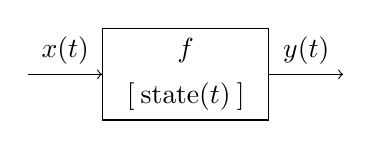
\begin{tikzpicture}[node distance=2cm]
\node[signal function with state] (arrf) {$f$ \nodepart{second} $[\: \operatorname{state}(t) \: ]$};
\coordinate[left of=arrf] (in);
\coordinate[right of=arrf] (out);
\draw [->] (in) to node[auto] {$x(t)$} (arrf);
\draw [->] (arrf) to node[auto] {$y(t)$} (out);
\end{tikzpicture}
\captionof{figure}{Signal function}
\label{fig:sigfunc}
\end{figure}

\section{FRP frameworks}
\label{sec:frameworks}
\subsection{Netwire}
Not sure if we want to keep this.
\subsection{Elm}

\section{A functional game}
\label{sec:game}

\section{Related works}
\label{sec:related}
Conal Elliott's paper "Push-pull functional reactive programming" \cite{Elliott2009-push-pull-frp} serves an integral role in modern FRP
and serves as the theoretical basis of many FRP libraries. Alexander Berntsen master thesis on programming game systems in Haskell \cite{Berntsen2014-game-systems-haskell} compares imperative and functional game design based on a medium-sized game and provides substantial evidence supporting the usage of strongly static typed purely functional programming for game development. Charles' post about recreating Asteroids in Netwire \cite{asteroids} describes difficulties encountered when implementing a game using Netwire.
\section{Conclusion and Outlook}
\label{sec:conclusion}

\bibliographystyle{plain}
\bibliography{references}
\end{document}
